\section{HTML minimizer}\label{sec:html_minimizer}

The HTML minimizer module is responsible for removing boilerplate content from the crawled HTML pages, retaining only the relevant content for further processing.
This module is crucial for improving the efficiency and accuracy of the subsequent page classification and information extraction tasks.
The minimizer works by analyzing the structure of the HTML page and identifying the main content areas, while discarding headers, footers, advertisements, and other non-essential elements.
This process reduces the amount of data that needs to be processed and helps focus the extraction algorithms on the most relevant parts of the page.
The benefits of minimizing a page before processing include:
\begin{itemize}
    \item \textbf{Improved accuracy:} By removing irrelevant content, the minimizer helps the subsequent modules focus on the most relevant parts of the page, leading to more accurate classification and extraction results.
    \item \textbf{Reduced processing time:} Minimizing the HTML pages reduces the amount of data that needs to be processed, which can lead to faster processing times and improved system performance.
    \item \textbf{Reduced cost:} Minimizing the HTML pages reduces the amount of data that needs to be processed, which can lead to lower operational costs.
    \item \textbf{Lower storage usage:} By reducing the size of the HTML pages, the minimizer can help lower memory and storage requirements, making the system more efficient and cost-effective.
\end{itemize}

The HTML minimizer module consists of two main subcomponents:
\begin{itemize}
    \item \textbf{Boilerplate removal library}: This is a library written in Python, which implements a variation of the site style trees algorithm for boilerplate removal.
    This package is published on PyPI\footnote{\url{https://pypi.org/project/boilerplate-remover/}} and can be installed using pip.
    \item \textbf{HTML minimizer workers}: These are AWS ECS tasks which run on a schedule.
    On each run, they fetch all pages which have been crawled but not yet minimized, and process them using the boilerplate removal library.
    The minimized pages are then stored in an S3 bucket for further processing by the page classifier, information extractor, and product matching modules.
\end{itemize}

\subsection{Boilerplate removal library}\label{subsec:boilerplate_removal_library}

This library implements a variation of the site style trees algorithm for boilerplate removal.
Given the HTML content from a web page, the library first runs a pre-processing step to clean the HTML and remove any unnecessary elements, such as scripts and styles.
Next, it constructs a site style tree for each page, which represents the hierarchical structure of the page's content.
Figure \ref{fig:site_style_tree} illustrates how a site style tree is constructed from the HTML content of a web page.

\begin{figure}[H]
    \centering
    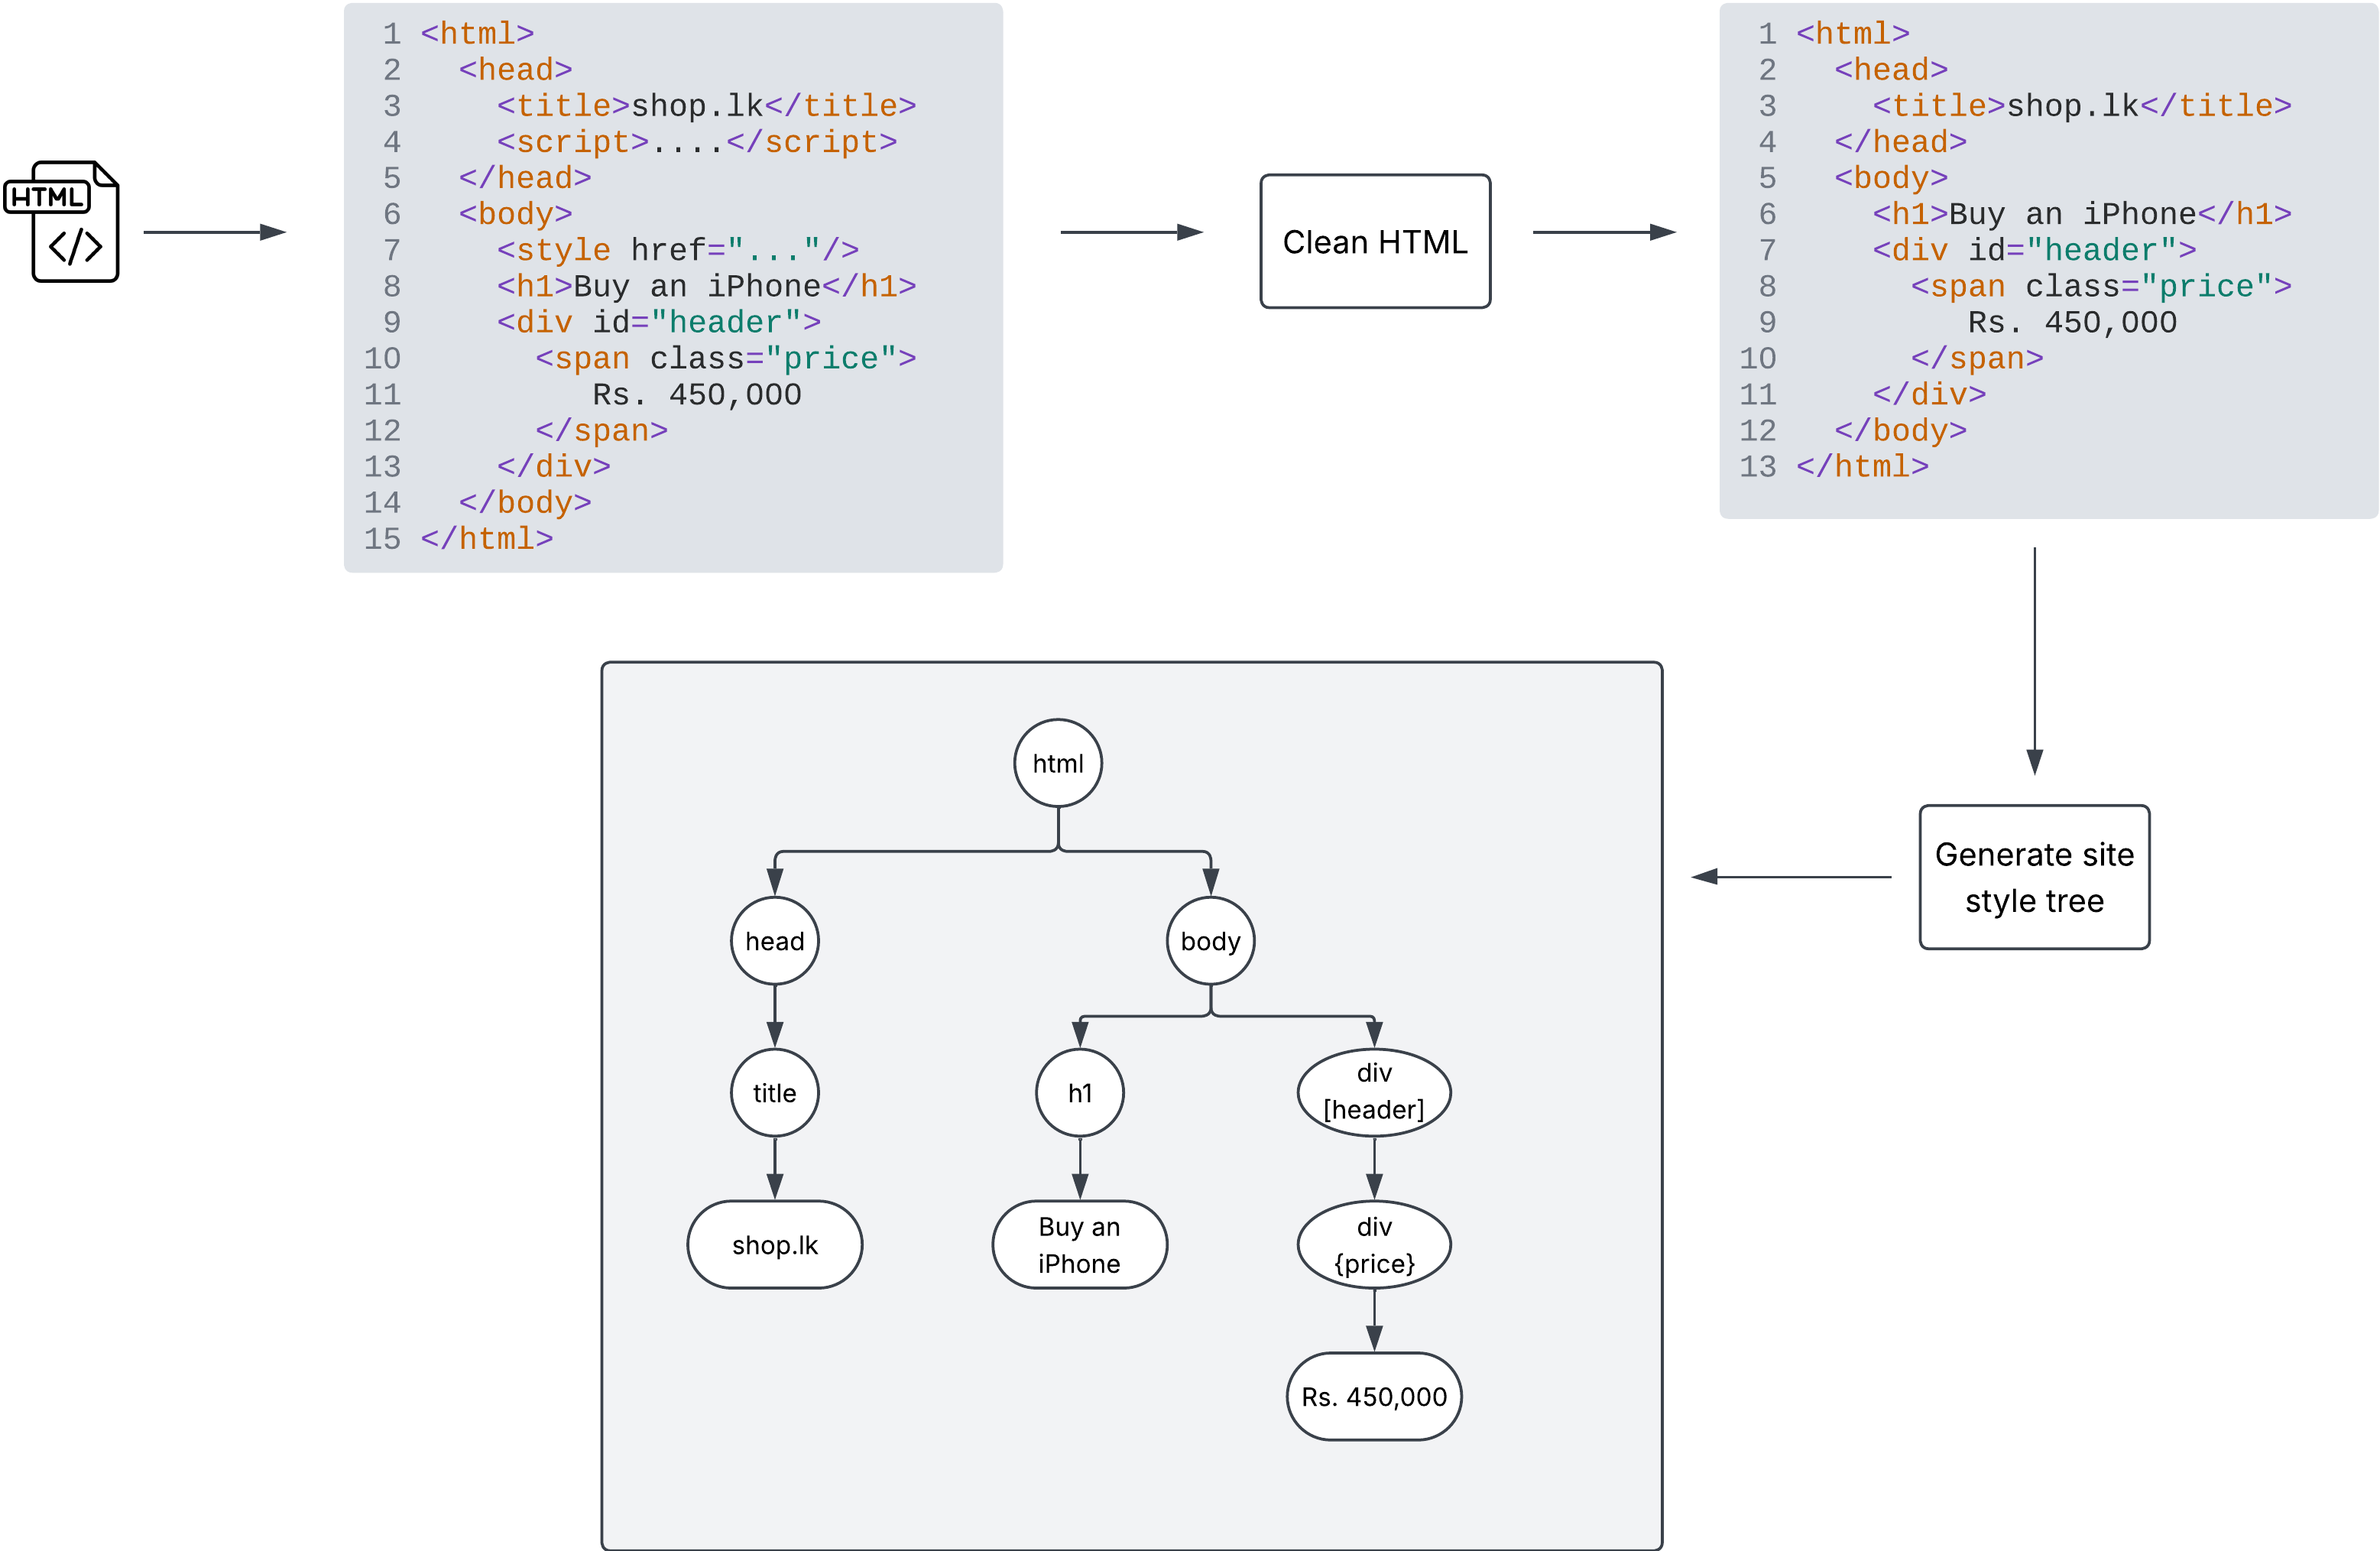
\includegraphics[width=0.8\textwidth]{images/site_style_trees_generation}
    \caption{Simple example of site style tree construction from HTML content.}
    \label{fig:site_style_tree}
\end{figure}

Then, these individual site style trees are merged to create a single site style tree that captures the common structure of the pages.

Each node in the tree contains the following attributes:
\begin{itemize}
    \item \textbf{Tag name:} The HTML tag name of the node (e.g., div, p, h1).
    \item \textbf{ID:} The unique identifier of the node, if any (e.g., id attribute).
    \item \textbf{Text content:} The text content of the node, if any.
    \item \textbf{Children:} A list of child nodes, representing the nested structure of the HTML elements.
    \item \textbf{Count:} The number of times this node appears in the set of HTML pages.
\end{itemize}

If a node has a high count, it indicates that the node is common across multiple pages and is likely to be boilerplate content.

Finally, all nodes with a count below a certain predefined threshold are removed from the tree, as they are considered to not be boilerplate content.
The remaining tree structure then becomes the \texbf{anchor tree}, which is a representation of the common structure of the pages.
Figure~\ref{fig:anchor_tree} illustrates how an anchor tree is constructed from a collection of site style trees.

\begin{figure}[H]
    \centering
    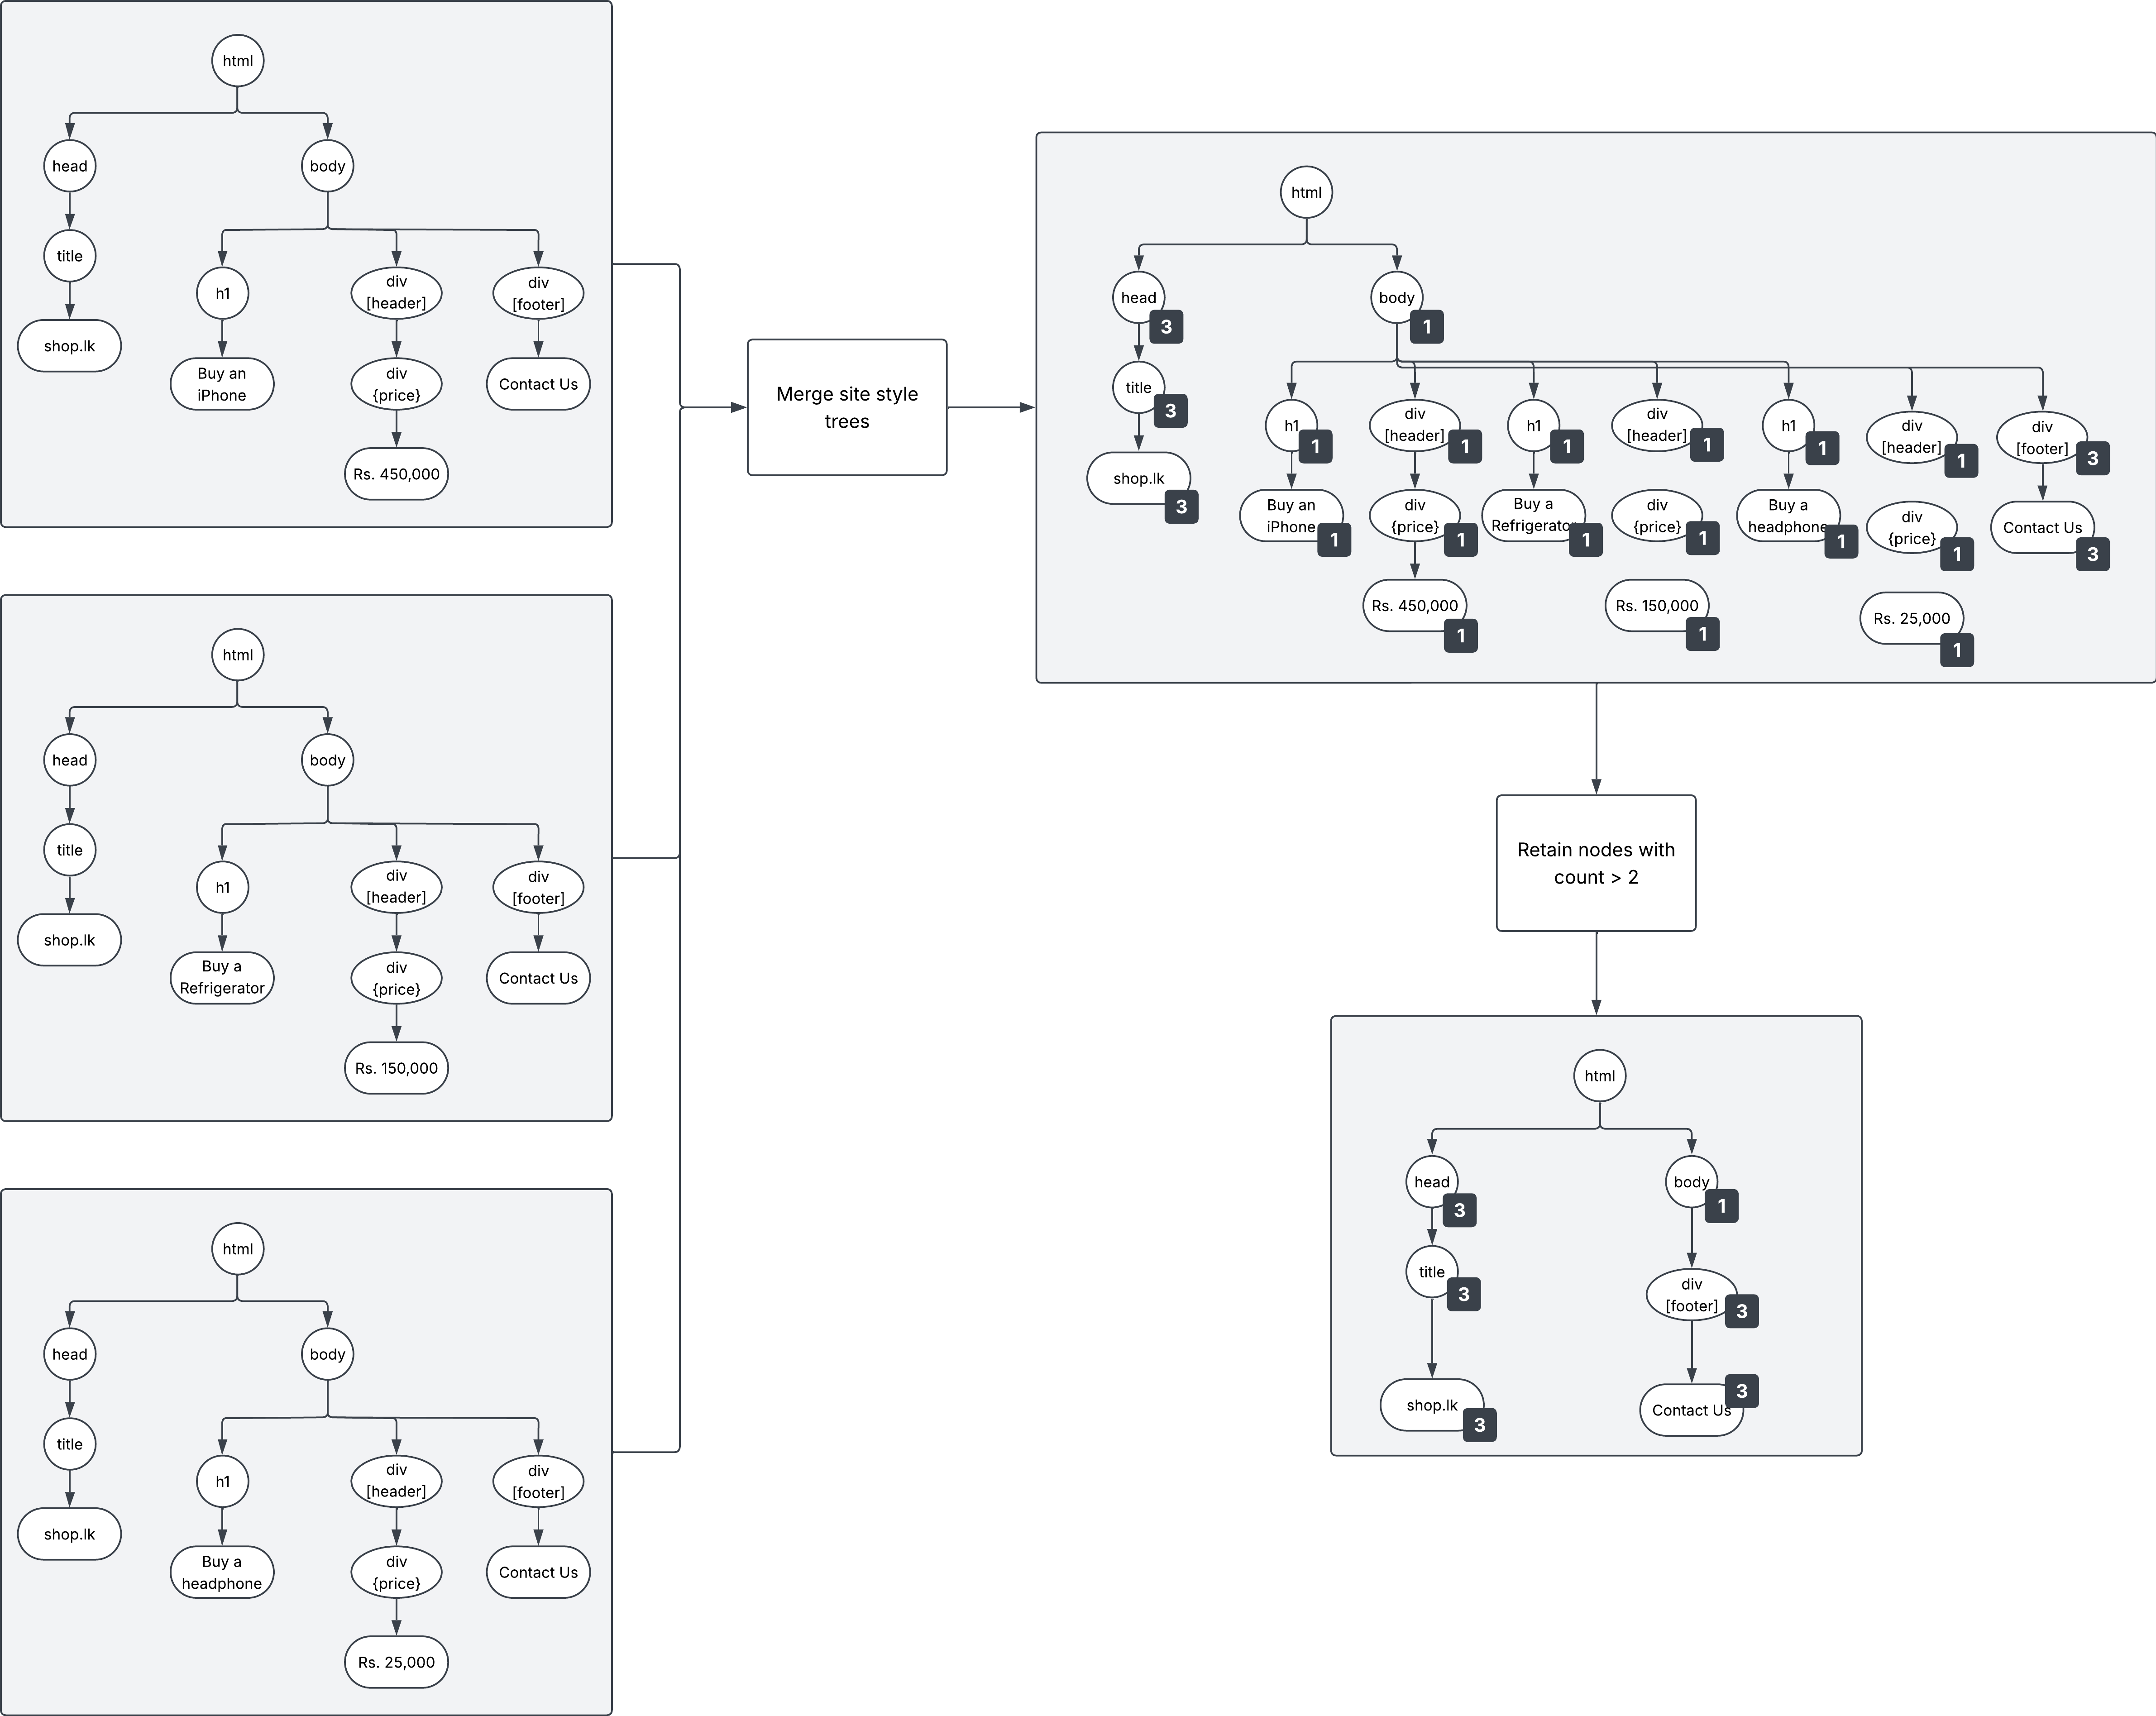
\includegraphics[width=1\textwidth]{images/anchor_tree_generation}
    \caption{Simple example of anchor tree construction from a collection of site style trees.}
    \label{fig:anchor_tree}
\end{figure}

When a new page is processed, its site style tree is compared to the anchor tree.
Nodes that match the anchor tree are considered to be boilerplate content and are removed from the page.
The remaining nodes are considered to be the main content of the page and are retained.
The processed tree is passed to a post-processing step, which reconstructs the HTML page with only the relevant content, and the minimized HTML is returned.